
% ==========================================
\section{Controlled experiments}
\label{Synthetic_exp}

With the goal of finding the regime of hyper parameters and optimization techniques where multi-region demixing works best , we start with a series of experiment where we mixed known expression profiles in a controlled way. This allowed us to solve mulit-region demixing in a settings where the latent factors are known and used as a ground truth. We first describe how the dataset was created and then characterize how performance depends on the number of samples and the number of latent factors (cell types).

\subsubsection*{Creating the mixture dataset}
We created controlled mixtures from a set of real transcriptome measurements, measured using microarrays from isolated cells. \citet{okaty2011cell} have collected 195 cell-type-specific profiles from 64 cell types spanning multiple regions and layers of the mouse brain. These profiles were previously measured after isolating cell using varous tehcniques (FACS, LMD).
 
Specifically, we create the known latent factors by collecting profiles for the 3 major population of cell types in the brain: neurons, astrocytes and oligodendrocytes. Each profile $\c$ is represented by 14580 genes. Profiles were extracted from 7 brain regions:  cortex layer 5A, cortex layer 5B, cortex layer 6, striatum, cerebellum, brainstem and the spinal cord. For each of these region, we also found the proportions of the three cell types reported in the literature \cite{Herculano2014}. (cortex:  0.7,0.1,0.2 for neuron, astrocytes, oligodendrocytes; cerebellum: 0.5,0.15,0.35, other: 0.65,0.1,0.25).

To draw a mixture sample, we drew proportion values $p_{neuron},p_{astro},p_{oligo}$ by adding multiplicative noise to the literature proportions. Each proportion was multiplied by a random value in [0,1] and scaled back to a  sum of 1. Finally, we added multiplicative Gaussian noise to the expression level of all genes, of the form $N(1,\xi^2)$, with noise levels of $\xi=10\%$ and $\xi=1\% $.

We then used the known mixtures to test the quality of reconstructed profiles as a function of number of samples, noise level, number of factors, and the optimization algorithm. 



%We evaluated the reconstructed profiles by computing their %spearman correlation with the true profiles. We then, %matched the best true profiles to the reconstructed %profiles.

%Each time we sampled n noisy samples and reconstructed the %profiles using these samples. The error bars in figure  %represented the sem over 30 repetitions.  

% \subsubsection*{bench-marking optimization method for single region NMF}

Since NMF is a non-convex problem different optimization techniques often reach different local minimas even when initialized using the same starting points. These differences in performance can result from the method of choice for each iteration (MM or ALS) or from the stopping and convergence rates of each alteration (in the ALS). We benchmarked 4 optimization techniques on data taken from a single region and found that all performed better with more samples. When the number of sample is sufficiently large we did not observe much difference in the performance of the different methods. while in a small number of samples the block-pivoting and the active-set performed slightly better (both had the same level of performance, and their graph overlaps) Figure \ref{fig:controlled_exp}(a).

%\subsubsection*{analyzing number of samples}
Next, we applied our multi-region demix to the controlled data from the 7 brain regions.
In the regime where only limited samples are available, there is sweet spot where we improve over the naive cases by using the connection between regions. As we increase the number of samples the benefit that we gain by using our method diminishes Figure \ref{fig:controlled_exp}(b). With enough samples solving the individual problems performs almost just as well. 


\begin{figure}[!hbt]
   (a) \hspace{120pt}(b) \hspace{120pt}(c) \hspace{120pt}
   \centering
     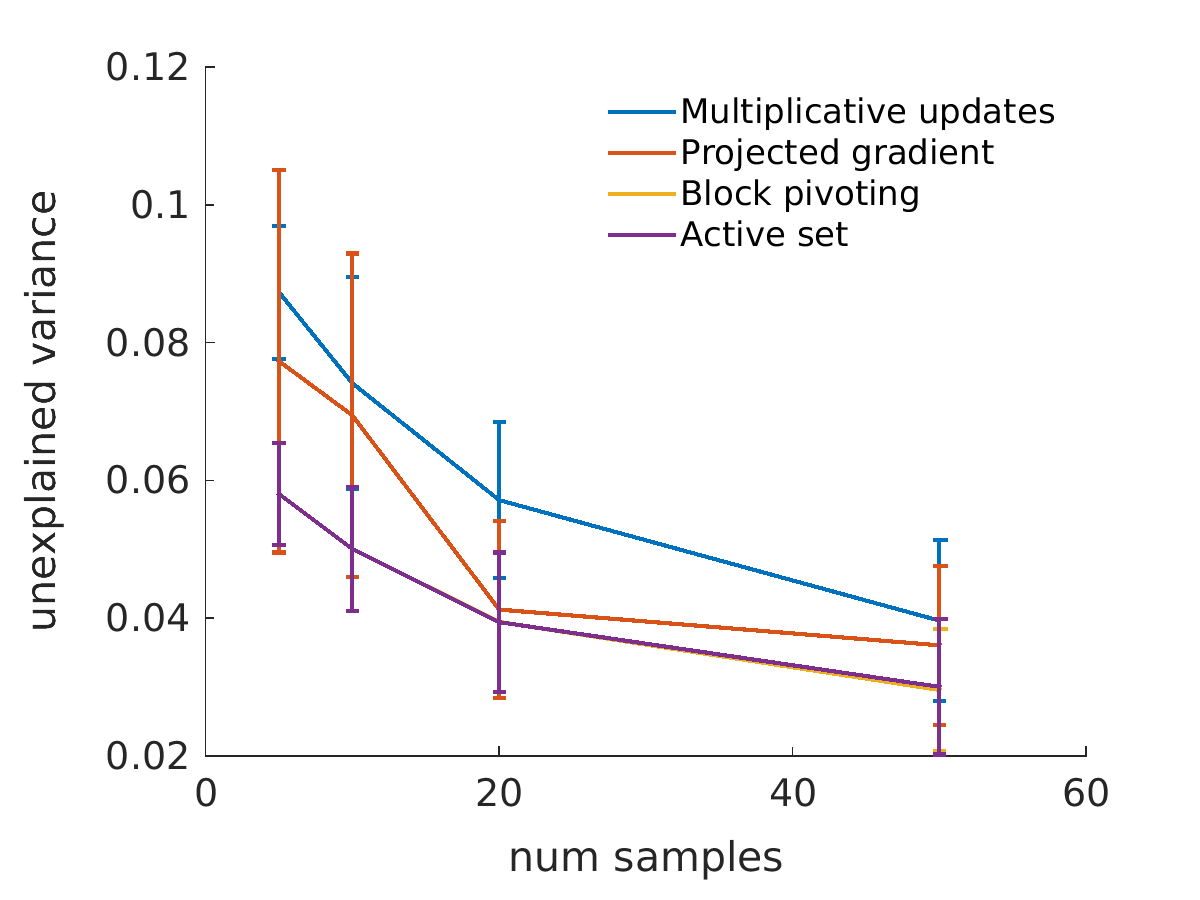
\includegraphics[width=0.32\textwidth]{methods}
     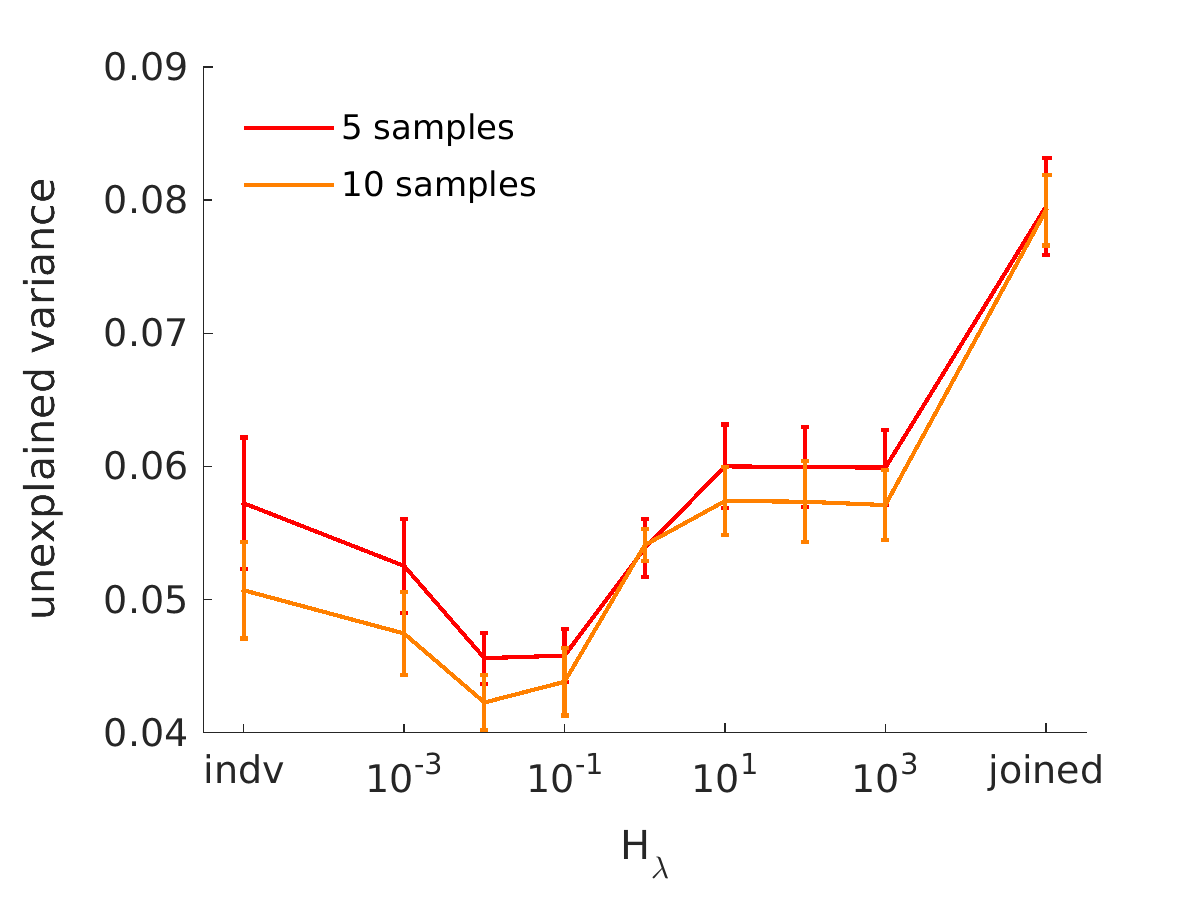
\includegraphics[width=0.32\textwidth]{lambda_samples}
     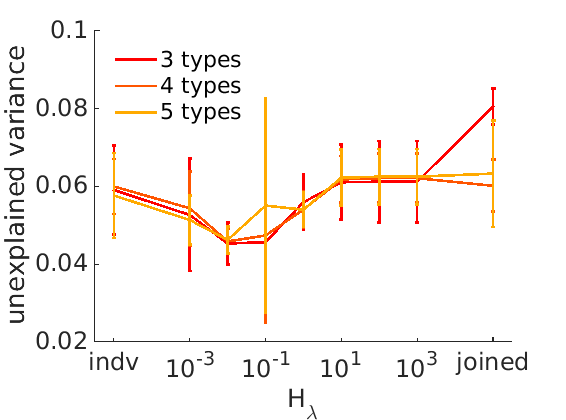
\includegraphics[width=0.32\textwidth]{num_types}
    \caption{Demixing in controlled experiments. 
    {\bf{(a)}}  Within a single region, all optimization methods improve when using more samples. The {\em active set} approach and the {\em block pivoting} outperformed other methods, particularly with few samples. {\bf{(b)}} Soft-sharing of latent factors lead to improved reconstruction in the multi-region settings, particularly with few samples. {\bf{(c)}} Reconstruction using more cell types then needed does not improve the results.} 
    \label{fig:controlled_exp}
\end{figure}

{\bf{LIOR, HOW MANY REGIONS IN FIGURE 2B?        - 7, I mentioned this above, in the creation of the dataset, is there anyplace you want to mention this again ?}}

%\subsubsection*{analyzing number of cell types}

As we increase the number of types the we are able to numerically better reconstruct the data matrix because we are allowing an approximation with of a larger rank. After we perform the demixing we match the best demixed profiles with true profile. This can improve the score since we can overfit. However, we did not notice any gain by using the extra profiles. It seems like it recovered the original profiles and some other vectors which helped to lower the overall fit but not the correlation to the original profiles. Overall it seems that this coincide with Ockham's razor and we can select simplest model which still capture the data \ref{fig:controlled_exp}(c). 


We found that the use of priors was somewhat fragile. While prior that were taken from the same experiment helped to imporve the score, priors of the same cell type just gathered in different experiments lowered our demixing success. 


% ==========================================
\section{Experiments with postmortem human brain expression}
\label{Human_exp}

We turn to analyze real mixtures collected using RNA-seq measurements from postmortem human brains. We used data from brainspan \cite{brainspan} (\url{http://www.brainspan.org/} and limited analysis to donors older than 17 years, leaving 8 adult human donors. We therefore had eight samples from each brain region. Each expression profile is represented by a vector of 52376 measurements including transcripts counts for coding and non-coding sequences. 

%Collecting human brain measurements is not easy to task since the the tissues has to be extracted not long after the subject death. So while the expression in each tissue can be represented in more details with the advancement of the sequencing tools, the number of samples is still extremely limited. For example, in our dataset there only few dozen samples and each is representation by tens of thousands features.

RNA sequencing is becoming the main way to measure gene expression in tissues, replacing the older microarrays technology. RNA sequencing provides more quantitative measurement since it actually counts the number of RNA transcripts in a tissue, as opposed to the more qualitative microarrays measurements. As such, RNA-seq data is more suitable for demixing since the number of RNAs transcripts grows linearly with the proportion of correspondiong cells in the tissue.

To evaluate the quality of demixing, we compare the inferred hidden cell-type specific profiles to transcriptome profiles measured in population of cells sorted by their cell type. At the time we conducted the analysis the cell-type specific RNA-seq data were only available in mouse \cite{barres2014}. We mapped the genes in the human to their orthologs in mouse and computed the spearman correlation between the reconstructed profiles and each of the single cell profiles. Recently such cell-type-specific data was made available for human, which will allow us to perform better validations. 

We determined the strengths of region-to-region relatedness $\phi_{r,s}$ based on the brain-region-ontology described in Figure \ref{fig:bro}. To verify that the human transcriptome measurements agree with this ontology, we first used an agglomerate hierarchical clustering over regions, by clustering expression profiles of these regions collected using microarray data by \cite{kang2011spatio}. The resulting region hierarchy had very string agreement with the brain region ontology, consistent with previous reports that adult expression patterns reflect brain development \cite{zapala2005}. The strengths of region-to-region attractive potentials $\lambda_{r,s}$ was determined as $\lambda \phi_{r,s}$ where $\lambda$ is a hyper parameter controlling the overall weight of edge potentials. 


Figure 3 shows the residual variance computed based on a Spearman correlation between the predicted and ground truth profiles, for three cell types and 5 brain regions. The details of the evaluation procedure was explained in section 5 above. We selected the 5 brain regions by selecting 3 subcortical regions and 2 cortical regions that were most remote (dorsolateral prefrontal cortex and primary visual cortex).

We compared our results with those of random baseline that was obtained by repeatedly selecting a set of 3 samples as the reconstructed profiles. It should be notated that even single cell experiments that are gathered from the same species in different experiment and from different region is only correlated to the other samples from the same type by 0.877. 
We notice that for most parts we are able to improve the reconstruction over the baseline. The use of the regions prior also improves the demixing over the demixing obtained using each brain region individually.


%   We find that in our reconstructed profiles the gene that are
%   For each of demixed profiles we performed enrichment analysis and found that ...



\begin{figure}[!hbt]
    \label{fig:human}
   (a) \hspace{120pt}(b) \hspace{120pt}(c) \hspace{120pt}
   \centering
     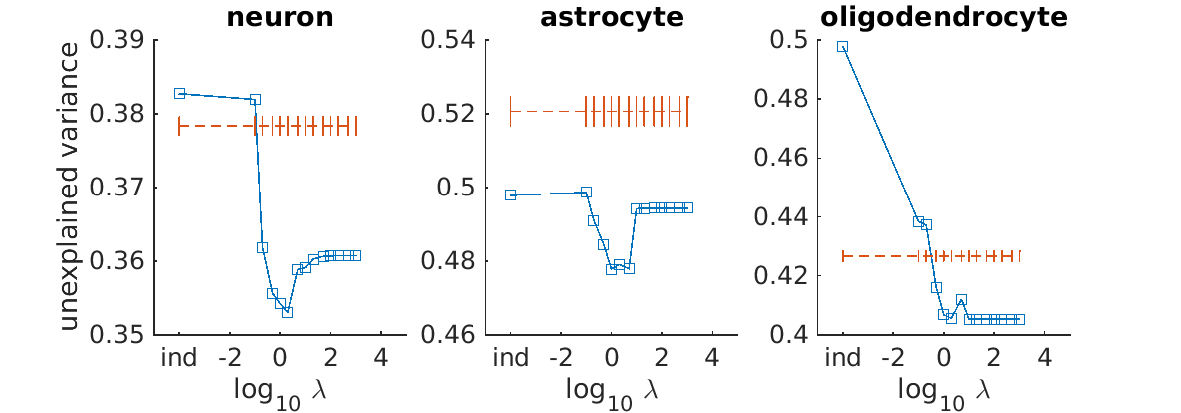
\includegraphics[width=0.99\textwidth]{3panels_var_AMY-CBC-DFC-HIP-V1C.png}
     \caption{Demixing RNA-seq data from 5 human brain regions \cite{brainspan}. Blue curve and squares correspond to the residual variance $(1-\rho^2)$ as a function of the strength of attractive region-to-region potentials $\lambda$. Red dashed line corresponds to a best-matched-sampels baseline (see text). At the optimum, the residual unexplained variance is reduced by 7\% for neurons, 8\% for astrocytes and 5\% in oligodendrocytes.}
    
\end{figure}


% [Add in the human experiment section We first verified that the brain regions in our data agree with the dev ontology: we clustered the brain regions in a hierarchical way and compared the resulting hierarchy to the dev ontology. We obtained very strong agreement …]. 
